\section{Story Diagrams and Story Patterns in a Nutshell (Jan and Dietrich)} \label{sec:Overview}

%- model-driven software development, raise abstraction level and use models instead of code as the key artifact
%- specify structure and behavior of the software under development, make the models runnable/executable
%- UML offers notations for description of software structure and development, esp. class and activity diagrams
%- activity diagrams are too informal to be automatically executed (natural language used)
%- we replaced the informal activity descriptions with formal descriptions of operations on object structures and developed a new formal language called story diagrams

%- story diagrams are special UML activity diagrams
%- developed to formalize the description of a software's behavior (UML activity diagrams usually use informal textual descriptions of the tasks to be performed)
%- motivation: complete specification of a software, structure and behavior, i.e. make the software specification executable (code generation and interpretation)

In model-driven software development, a software model is the key artifact under development.
It describes the software structure as well as its behavior and 
can be translated to runnable source code or be interpreted to be executed.
The UML offers notations for the description of the software structure and behavior,
besides others class diagrams and activity diagrams.
Since UML activity diagrams use natural language to describe the software's behavior,
a formal behavioral specification is needed to make the software model executable.
For that purpose \emph{story diagrams} have been developed \cite{FNTZ00}.
They refine UML activity diagrams and replace the natural language with a formal language to specify behavior
and, thus, can be automatically executed.

%- motivation: (formally) describe modifications of object structures for object-oriented software systems
%- use a graphical notation to specify operations on object structures (object structure modifications), OO world
%- each operation describes a modification of a given object structure, basically the modifactions are creations and removals of objects and their interconnections
%- graphically describe the object structure to be modified, mark the elements to be created and those to be removed

Story diagrams describe the control flow similar to UML activity diagrams by means of activity nodes and activity edges.
The behavior of each activity node is described using a graph transformation language called \emph{story patterns}.
Each activity node embeds a story pattern.
A story pattern uses a graphical notation to specify modifications of object structures in object-oriented software systems.
The modifications are basically creations and removals of objects and their interconnections (links).

%- motivation: use an appropriate, familiar, and simple notation for object structure modifications; we use a notation similar to UML object diagrams
%- motivation: declaratively describe the operations in activity nodes, thus, reduce complexity (avoid describing how to perform the operations)
%- motivation: keep determinism to a certain extent to specify the conditions for and the order of object structure modifications

To use a simple and familiar notation, story patterns are similar to UML object diagrams.
A story pattern represents an object structure to be modified and includes annotations specifying which objects and links are to be removed and created.
Story patterns are a declarative language, since they only specify what to remove and create, but not how and in which order.
This way the complexity of the behavioral specifications is reduced.
In contrast to the deterministic control flow specified by activity nodes and edges that determine the order of story pattern executions,
the order of creations and deletions specified by a story pattern is non-deterministic.

%- motivation: base the specification on a well-known formalism (for execution and analyses)
%- story diagrams use graph transformations in their activity nodes (well-known formalism, exhaust the given theories for analyses and execution)

Story patterns base on \emph{graph grammars}, a well-known formalism and corresponding theories \cite{Roz97}.
Thus, precise analyses of the operations described by story patterns are possible,
e.g., it can be checked if certain properties of the object structure to be modified remain after the structure's modification.

%- given a so called host graph (an object structure or model), story diagrams describe the graph's modifications by means of creating or removing nodes and edges (objects and links)
%- the host graph, in our case, is a typed attributed graph, i.e. we have a graph to be modified (object structure, token model) and a corresponding type graph (type model or meta-model) describing the types and properties of the objects in our host graph
%- a graph transformation is executed by identifying a subgraph in the host graph which corresponds to the graph specified in the transformation (matching, subgraph isomorphism), removing nodes and links that are marked to be removed, and creating new nodes and links that are marked to be created

A story pattern specifies a graph transformation \cite{Roz97}.
Given a so-called \emph{host graph}, the graph to be modified, a graph transformation removes and creates nodes and edges in the given host graph.
The host graph is a typed attributed graph, i.e. there is a type graph determining the types and attributes of the nodes.
A graph transformation is executed on a host graph by identifying a subgraph in the host graph that is similar to the one specified in the graph transformation and then removing and adding the specified nodes and edges.
The identification of the subgraph for modification is called \emph{graph matching} and includes the \emph{subgraph isomorphism} problem.

In case of story patterns, the host graph is the object structure or model to be modified (\emph{token model}) \cite{Kue06},
i.e. the run-time data of the executed software.
The type graph is a set of classes and their relations which define all potential object structures at run-time.
These classes and relations are a so-called \emph{type model} or meta-model \cite{Kue06}.
They are required to specify story patterns.

For example, the class diagram in Figure~\ref{fig:SDExampleClassDiagram} defines the types \fe{Class} and \fe{Attribute} as well as their relations, attributes, and operations.
The corresponding story diagram in Figure~\ref{fig:SDExampleStoryDiagram} definies the behavior of the \fe{removeAttribute} method defined in the class diagram.
Here, the story diagram specifies that a class's attribute with the name given by the parameter \fe{text} is to be found in the class and in case of success this attribute is to be removed (\destroy).

\begin{figure}[htb]
	\centering
  \begin{minipage}[t]{.4\textwidth}
    \centering
    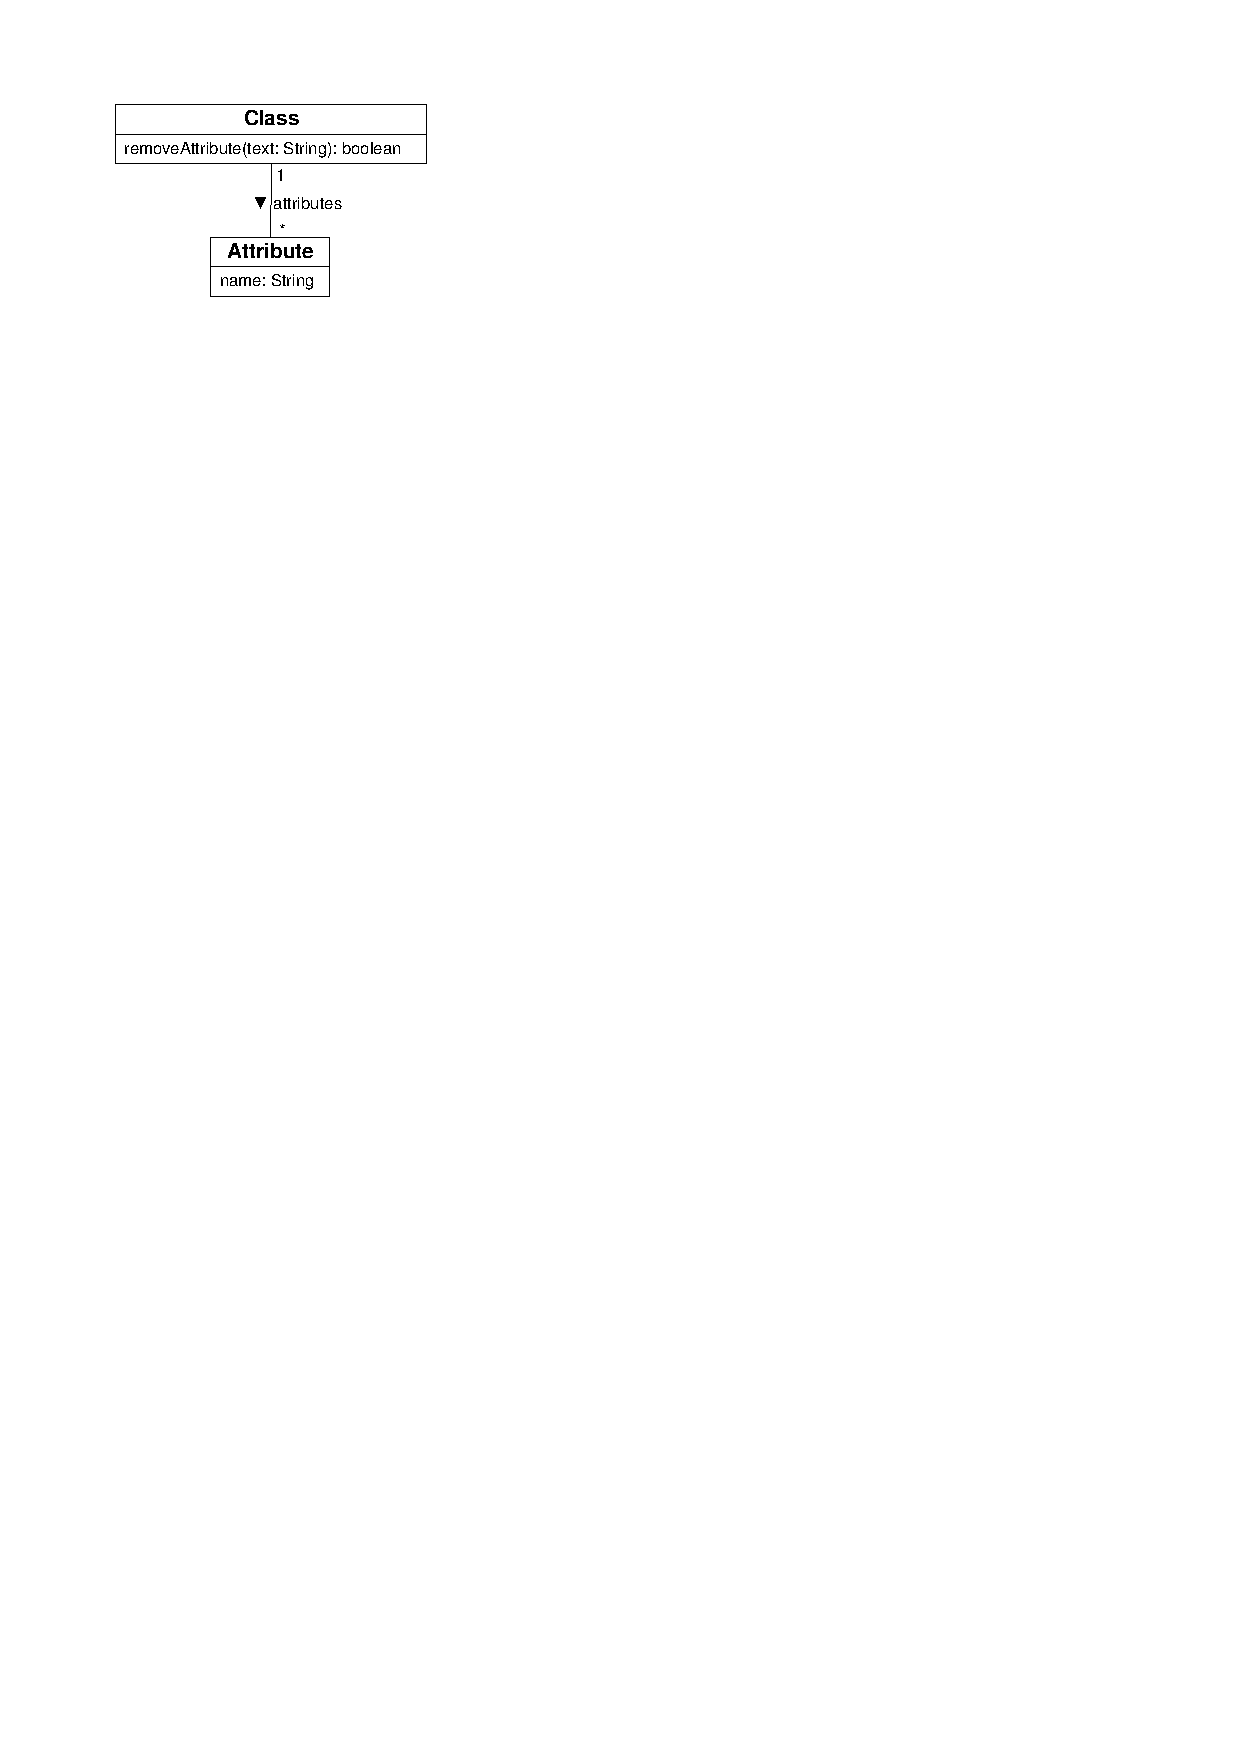
\includegraphics[scale=1]{SimpleSDRemoveAttributeClassDiagram} 
    \caption{Exemplary Type Model}
    \label{fig:SDExampleClassDiagram}
  \end{minipage}%
  \hfill
  \begin{minipage}[t]{.55\textwidth}
    \centering
    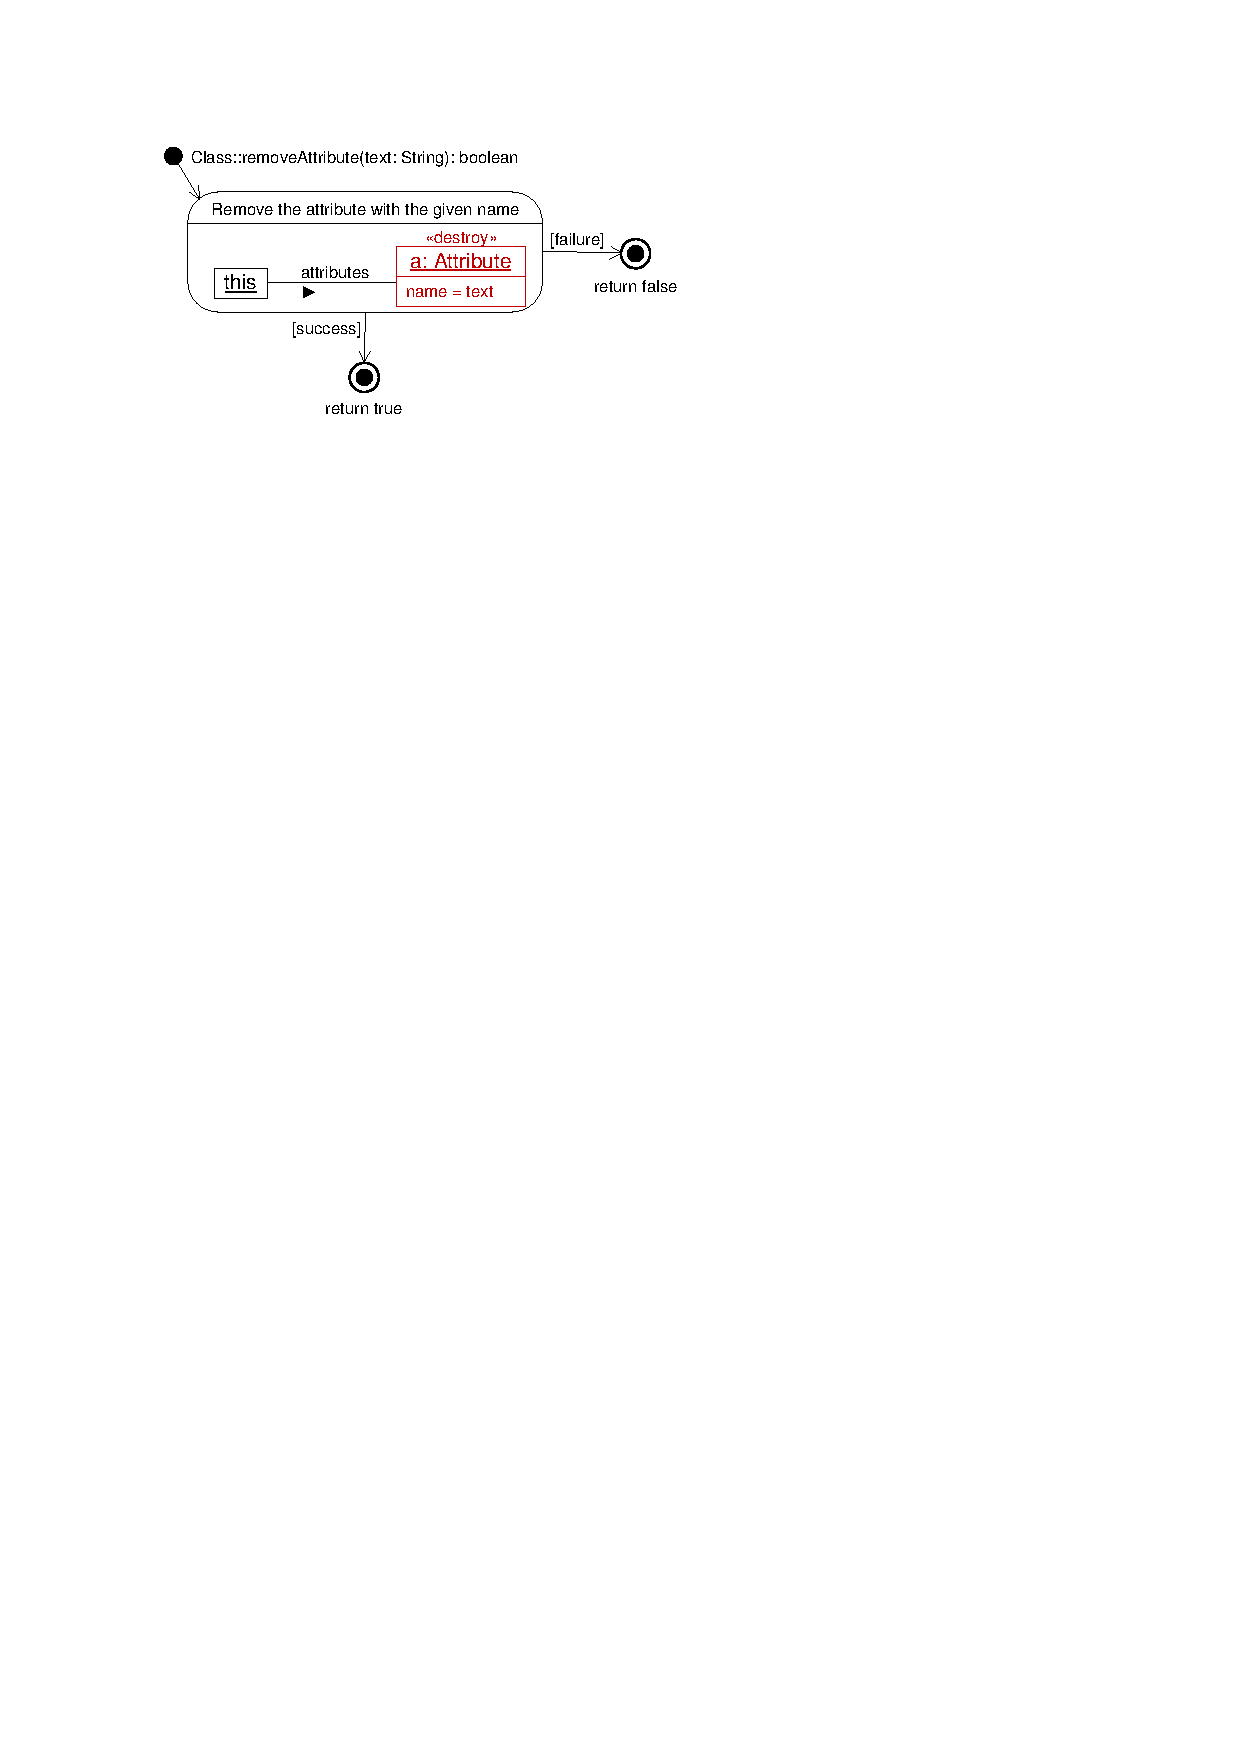
\includegraphics[scale=1]{SimpleSDRemoveAttribute}
    \caption{Exemplary Story Diagram}
    \label{fig:SDExampleStoryDiagram}
  \end{minipage}
\end{figure}

In summary, a story diagram is a special, formally defined UML activity diagram
that embeds graph transformations, so-called story patterns, in its activity nodes
to precisely describe run-time behavior by means of graph transformations.

%\subsection{Application scenarios (?)} \label{sec:Applications}